\documentclass[norsk,a4paper,12pt]{article}
\usepackage[utf8]{inputenc}
\usepackage{graphicx} %for å inkludere grafikk
\usepackage{verbatim} %for å inkludere filer med tegn LaTeX ikke liker
\usepackage{amsmath}
\usepackage{float}
\usepackage{color}
\usepackage{listings}
\usepackage{hyperref}
\lstset{language=c++}
\lstset{basicstyle=\small}
\lstset{backgroundcolor=\color{white}}
\lstset{frame=single}
\lstset{stringstyle=\ttfamily}
\lstset{keywordstyle=\color{red}\bfseries}
\lstset{commentstyle=\itshape\color{blue}}
\lstset{showspaces=false}
\lstset{showstringspaces=false}
\lstset{showtabs=false}
\lstset{breaklines}
\lstset{postbreak=\raisebox{0ex}[0ex][0ex]{\ensuremath{\color{red}\hookrightarrow\space}}}


\title{FYS3150 - Computational Physics\\\vspace{2mm} \Large{Project 2}}
\author{\large Richard Fauli\\ Dorthea Gjestvang\\ Even Nordhagen}
\date{\today}
\begin{document}

\maketitle

\begin{abstract}
\end{abstract}
\begin{itemize}
\item Github repository containing programs and results are in: \url{https://github.com/richaraf/Comphys_projects/tree/master/Project_2}
\end{itemize}
\section{Introduction}
In this project, we study the theory behind quantum dots, a highly relevant subject in modern physics. A quantum dot is one or two electrons trapped in an quantum well. These are often referred to as arificial atoms, as they, like natural atoms, have discrete energy levels. (Reference: http://www.nature.com/nature/journal/v379/n6564/pdf/379413a0.pdf)\par
\vspace{3mm}

Our goal in this project is to simulate a quantum dot, modelled as one or two electrons bound in a three-dimensional harmonic oscillator well. Quantum Mechanics tells us that we find the behaviour of these electrons by solving the radial equation with the harmonic oscillator potential, $V(r) = \frac{1}{2}m^2\omega^2r^2$:

\begin{equation}
    - \frac{\hbar^2}{2m}(\frac{1}{r^2}\frac{d^2}{dr^2}r^2\frac{d}{dr} - \frac{l(l+1)}{r^2})R(r) + \frac{1}{2}m\omega^2r^2R(r) = ER(r)
\end{equation}
\vspace{3mm}

We do so by rewriting equation (1) with dimensionless variables, and reduce the equation to a single eigenvalue problem, which we solve by implementing Jacobi's rotation method. Thereafter, we compare the obtained wave functions for one and two electrons, and interpret the results physically. We also examine what effect the strength of the harmonic potential has on the wave function in the two-electron case.

\section{Theory}
\subsection{One electron}
To solve the Schroedinger's equation (SE) for one electron in a three-dimensional harmic oscillator well, we first assume spherical symmetry, which means we only need to solve the radial part of SE
\begin{equation}
-\frac{\hbar ^2}{2m}\left(\frac{1}{r^2}\frac{d}{dr}r^2\frac{d}{dr} - \frac{l(l+1)}{r^2}\right)R(r) + V(r)R(r) = ER(r),
\label{eq:SEradialgeneral}
\end{equation}
where $\hbar = 6.582 \cdot 10^{-16}$ eV$\cdot$s, $m$ is the electron mass, $r \in [0,\infty)$ the radial distance, $V(r)$ is the potential, $E$ is the energy and $l$ is the orbital quantum number. For our harmonic oscillator the potential is $V(r) = (1/2)kr^2$, with $k=m\omega ^2$. If we look at the case where $l=0$, we get the energies to be $$E_n = \hbar \omega \left(2n + \frac{3}{2}\right).$$ If we also substitute $R(r) = (1/r)u(r)$ in equation (\ref{eq:SEradialgeneral}), the SE we want to solve becomes 
\begin{equation}
-\frac{\hbar ^2}{2m}\frac{d^2}{dr^2} u(r) + V(r) u(r) = Eu(r).
\label{eq:SEradial}
\end{equation}
We introduce the dimensionless variable $\rho = r/\alpha$, which means our potential becomes $V(\rho)= k\alpha ^2 \rho ^2 / 2$. Inserting $\rho$ and $V(\rho)$ into equation (\ref{eq:SEradial}) we get
$$-\frac{d^2}{d\rho ^2}u(\rho) + \frac{mk}{\hbar ^2}\alpha ^4 \rho^2 u(\rho) = \frac{2m\alpha ^2}{\hbar^2}Eu(\rho).$$
We can set $mk\alpha^4/\hbar^2 = 1$ and $2m\alpha^2E/\hbar^2 = \lambda$ which allows us the write the Schroedinger's equation as \begin{equation}
-\frac{d^2}{d\rho ^2}u(\rho) + \rho ^2 u(\rho) = \lambda u(\rho).
\label{eq:SEdimless}
\end{equation}
The second derivative can be expressed as $$u'' \approx \frac{u(\rho + h) - 2u(\rho) + u(\rho -h)}{h^2},$$ where $h$ is the step length. We use $N$ mesh points with $\rho_{min} = \rho_0$ and $\rho_{max} = \rho_N$ which means the step length is $h = (\rho_N - \rho_0)/N$. $\rho$ is discretized by 
\begin{align*}
\rho_i  = \rho _0 + ih && \text{with }i = 1,2,...,N,
\end{align*}
which means we can write our discretized SE as 
\begin{equation}
-\frac{u_{i+1}-2u_i + u_{i-1}}{h^2} + V_i^2u_i = \lambda u_i,
\label{eq:SEdiscretized}
\end{equation}
where $V_i=\rho_i^2$.
The discretized case in eq (\ref{eq:SEdiscretized}) can be written as a linear set of equations 
\begin{equation}
A\textbf{u} = \lambda \textbf{u},
\label{eq:Aulambdau}
\end{equation}
where A is the tridiagonal matrix
\setcounter{MaxMatrixCols}{20}
\begin{equation}
A=\begin{pmatrix}
\frac{2}{h^2} + V_1 && -\frac{1}{h^2} && 0 && ... && 0 && 0 \\
-\frac{1}{h^2} && \frac{2}{h^2} + V_2 && -\frac{1}{h^2} && ... && 0 && 0 \\
0 && -\frac{1}{h^2} && \frac{2}{h^2} + V_3 && ... && 0 && 0 \\
: && : && : && ^{\textbf{.}}. && : && : \\
0 && 0 && 0 && -\frac{1}{h^2} && \frac{2}{h^2} + V_{N-2} && -\frac{1}{h^2} \\
0 && 0 && 0 && 0 && -\frac{1}{h^2} && \frac{2}{h^2} + V_{N-1}
\end{pmatrix}
\label{eq:A}
\end{equation}
\subsection{Two electrons}
In the case of two electron without repulsive Coulomb interaction our SE is 
$$\left(-\frac{\hbar ^2}{2m}\frac{d^2}{dr_1^2} - \frac{\hbar ^2}{2m}\frac{d^2}{dr_2^2} + \frac{kr_1^2}{2} + \frac{kr_2^2}{2}\right)u(r_1,r_2) = E^{(2)}u(r_1,r_2),$$
where $E^{(2)}$ is the two-electron energy. Introducing a relative coordinate $\textbf{r} = \textbf{r}_1-\textbf{r}_2$ and the center-of-mass coordinate $\textbf{R} = (\textbf{r}_1 + \textbf{r}_2)/2$, we can write SE as
$$\left(-\frac{\hbar ^2}{m}\frac{d^2}{dr^2} - \frac{\hbar ^2}{4m}\frac{d^2}{dR^2} + \frac{kr^2}{4} + kR^2\right)u(r,R) = E^{(2)}u(r,R).$$


The energy can be split into relative energy $E_r$ and the center-of-mass energy $E_R$ as well as $u(r,R) = \psi(r) \phi(R)$. We can then separate the SE into an $r$-dependent part and an $R$-dependent part. The repulsive Coulomb interaction potential between the two electrons is expressed $$V(r_1,r_2) = \frac{\beta e^2}{|\textbf{r}_1-\textbf{r}_2|} = \frac{\beta e^2}{r},$$ where $\beta e^2 = 1.44$ eVnm. 

We are interested in solving the equation with $E_r$, because the $R$-dependent equation is very similar to the case of no repulsive Coulomb interaction. Adding the repulsive Coulomb potential the to $r$-dependent part of SE gives
$$\left(-\frac{\hbar ^2}{m}\frac{d^2}{dr^2} + \frac{kr^2}{4} + \frac{\beta e^2}{r}\right)\psi(r) = E_r\psi(r).$$ 
We again use the dimensionless variable $\rho = r/\alpha$ which gives us 
\begin{equation}
\left(-\frac{d^2}{d\rho ^2} + \frac{mk\alpha ^4 \rho ^2}{4\hbar ^2} + \frac{m\alpha \beta e^2}{\rho \hbar^2}\right)\psi(\rho) = \frac{m\alpha ^2}{\hbar^2}E_r\psi(\rho),
\label{eq:SEdimlessvars}
\end{equation}

which we can simplify and make look like equation (\ref{eq:SEdimless}) by fixing $\alpha$, defining a ''frequency'' $\omega _r$ and ''energy'' $\lambda_r$
\begin{align*}
\frac{m\alpha\beta e^2}{\hbar^2} = 1 && \omega_r^2 = \frac{mk\alpha^4}{4\hbar^2} && \lambda = \frac{m\alpha^2E}{\hbar^2}.
\end{align*}
The equation to solve then becomes \begin{equation}
-\frac{d^2}{d\rho ^2}\psi (\rho) + \omega_r^2\rho^2\psi(\rho) + \frac{1}{\rho}\psi(\rho) = \lambda \psi (\rho),
\label{eq:SEdimlessinteraction}
\end{equation}
which means we can write the potential for the interacting case as $$V_r(\rho) = \omega_r^2\rho^2 + \frac{1}{\rho}$$
and in discretized form $$V_{ir} = \omega_r^2\rho_i^2 + \frac{1}{\rho_i}.$$ The potential for the case where there is no interaction between the two electrons, we simply set $\beta$ to $0$, which means the potential becomes $$V_{nr}(\rho) = \omega_r^2 \rho^2,$$ which for discrete points can be expressed
$$V_{inr} = \omega_r^2\rho_i^2.$$
The eigenvalue-problem in equation (\ref{eq:SEdimlessinteraction}) can then be written as equation (\ref{eq:Aulambdau}), a set of linear equations, where $A$ is as defined in expression (\ref{eq:A}), with the potential $V_{ir}$ for the interacting case and $V_{inr}$ for the case without interaction.
\subsection{Conservation of dot product}
If we consider a set of vectors $\{\textbf{v}_i\}$, an orthogonal matrix U and the transformation $\textbf{w}_i = U\textbf{v}_i$. The dot product for our set of vectors an be expressed as $$\textbf{v}_j^T\textbf{v}_i,$$ which in the case of $\{\textbf{v}_i\}$ being an orthonormal basis means that $\textbf{v}_j^T\textbf{v}_i = \delta_{ij},$ where $\delta_{ij}$ is the Kronecker delta. The dot product of an orthogonal transformation is preserved
$$\textbf{w}_j^T \textbf{w}_i = (U\textbf{v}_j)^TU\textbf{v}_i = \textbf{v}_j^TU^TU\textbf{v}_i = \textbf{v}_j^T\textbf{v}_i,$$ which also means that orthogonality is preserved in the case where $\{\textbf{v}_i\}$ is an orthogonal basis.
\section{Method}
\subsection{Jacobi's method}
In this project we are using Jacobi's method, which transforms a matrix A into a diagonal matrix D with the eigenvalues of A on the diagonal. This is done by repeat setting the largest non-diagonal element equal to zero until all the non-diagonal elements are smaller than a tolerance $\varepsilon$. From linear algebra we know that a symmetric matrix always can be transformed into a diagonal matrix, so this should be valid for our specific symmetric matrix described in the theory. For doing this we need a transformation matrix S which sets the largest non-diagonal element to zero:
\begin{equation}
S^T A S=B
\end{equation}
Where B is the transformed A matrix where the largest non-diagonal element is set to zero. S is given by
\setcounter{MaxMatrixCols}{20}
\begin{equation}
S=\begin{pmatrix} 
1	&&0	&&\hdots		&&0		&&0	&&\hdots	&&0 	&&0\\
0	&&1		&&\hdots&&0&&0&&\hdots&&0&&0\\ \vdots&&\vdots&&\ddots&&\vdots&&\vdots&&\ddots&&\vdots&&\vdots\\ 0&&0&&\hdots&&cos\theta&&0&&\hdots&&0&&sin\theta\\
0&&0&&\hdots&&0&&1&&\hdots&&0&&0\\ \vdots&&\vdots&&\ddots&&\vdots&&\vdots&&\ddots&&\vdots&&\vdots\\ 0&&0&&\hdots&&0&&0&&\hdots&&1&&0\\
0&&0&&\hdots&&-sin\theta&&0&&\hdots&&0&&cos\theta\\
\end{pmatrix}
\end{equation}
where the locations of $sin\theta$ and $-sin\theta$ are depending on the indexes of the largest element of A. Therefore we first need to find this, something we can easily do numerically:
\begin{lstlisting}
max = 0;                     	//Largest element
for(k = [0,size A])
   for(l = [0,size A])
      if(k != l)		//Not on diagonal
         if(abs(A(k,l)) > max)
            kmax = k;		//Store indexes of
            lmax = l;		//largest element
            max = abs(A(k,l));
\end{lstlisting}
After the indexes of the largest element are found, we can start doing the Jacobi method (also called Jacobi rotation since the matrix S is a rotation matrix). By doing the multiplication $S^T AS = B$ for an arbitrary matrix A, we will see that B is constructed by
\begin{itemize}
\item $b_{ii}=a_{ii}\quad\quad\quad\quad\quad\quad\quad\quad\quad\quad\quad\quad\quad\quad\quad\quad\quad\quad\,\, i\not=k,\quad i\not= l$
\item $b_{ik}=a_{ik}cos\theta-a_{il}sin\theta\quad\quad\quad\quad\quad\quad\quad\quad\quad\quad\quad\quad i\not=k,\quad i\not= l$
\item $b_{il}=a_{il}cos\theta+a_{ik}sin\theta\quad\quad\quad\quad\quad\quad\quad\quad\quad\quad\quad\quad\, i\not=k,\quad i\not= l$
\item $b_{kk}=a_{kk}cos^2\theta-2a_{kl}cos\theta sin\theta +a_{ll}sin^2\theta$
\item $b_{ll}=a_{ll}cos^2\theta+2a_{kl}cos\theta sin\theta +a_{kk}sin^2\theta$
\item $b_{kl}=(a_{kk}-a_{ll})cos\theta sin\theta + a_{kl}(cos^2\theta sin^2\theta)$
\end{itemize}
where $i$ is an arbitrary columns or row index, $k$ is the index of the row with the largest non-diagonal number (in A) and $l$ is the index of the column with the largest non-diagonal number. This makes it easy to find B numerically, and by doing Jacobi's method on B a multiple times, the largest non-diagonal element will constantly be smaller. In the theory these elements should be equal to zero when the diagonal elements are equal to the exact eigenvalues, but we can get a good approximation of the eigenvalues even if the largest element is a small number. We implement this by choosing a small tolerance $\varepsilon$ and continue doing Jacobi's method until the largest element is smaller than this. The smaller $\varepsilon$ is, the better approach we have.\par\vspace{3mm}
The eigenvectors are found by
\begin{equation}
\textbf{w}_i=S\textbf{v}_i
\end{equation}
where \textbf{v} is a basis of eigenvectors, S is the transformation matrix and \textbf{w} are the eigenvectors of A. Numerically we are going to do this by updating the matrix R which is the identity matrix in the beginning. 
\begin{itemize}
\item $R_{il}=cos\theta r_{il}+sin\theta r_{ik}$
\item $R_{ik}=-sin\theta r_{il}+cos\theta r_{ik}$
\end{itemize}

\subsection{Solve the eigenproblem using Armadillo}
We are also finding the eigenvectors and eigenvalues with Armadillo, just to compare them with the eigenvalues and eigenvectors found by Jacobi's method. For a symmetric matrix, this is done by this script:
\begin{lstlisting}
vec eigval;
mat eigvec;
eig_sym(eigval, eigvec, A);
\end{lstlisting}
where we assume that armadillo is included. 

\subsection{Tests}
\subsubsection{Largest element test}
To ensure that the indexes of the non-diagonal largest element are found correctly, we have implemented a test for this. The test is a function which takes $k$ and $l$ as arguments (the indexes of the largest non-diagonal element) and placing the number 1 at this index while the remaining elements are zero. It will not allow us to place the element on the diagonal. Then we have a matrix where we know the exact location of the largest (non-diagonal) element. The next step is to send this matrix into the function which finds the largest element and returns the indexes of this. If this function returns the same indexes as where we placed the largest element, the largest element function passes the test.\par\vspace{3mm}
The reason why we want the test function to take the indexes as arguments, is to be able to vary the test matrix to ensure that the solver is not giving the right result accidentally.\par\vspace{3mm} 
We are also testing if the matrix sent into the largest element finder is quadratic. This is simply done by comparing the number of rows and the number of columns. The test raises an error if the matrix is not quadratic.

\subsubsection{Check of orthogonality}
The eigenvectors should be orthogonal since they cannot be linear combination of each other. This means that the inner product between two different eigenvectors needs to be zero. The mathematical expression can be written as
\begin{equation}
\langle \textbf{v}_i|\textbf{v}_j\rangle =
    \begin{cases}
            c, &         \text{if } i=j,\\
            0, &         \text{if } i\neq j.
    \end{cases}
\end{equation}
where $c$ is a constant. We are not interested in $c$, but we want to check if the inner product between two \textit{different} vectors are zero. The test loops over all the different combinations of eigenvectors (but not equal eigenvectors), and takes the inner product between them. Thereafter it compares the inner product with a given tolerance, and the test passes as long as the inner product is smaller than the tolerance.

\section{Results}

\subsection{Run time}
\par
\vspace{3mm}
We ran our program for different numbers of grid points N, and noted the run times of our Jacobi rotation algorithm and the armadillo solver. The run times are presented in Table 1. 
\par
\vspace{3mm}


Table 1: Run time of our Jacobi-algorithm vs the Armadillo solver\par
\vspace{3mm}

\begin{tabular}{|c|c|c|}\hline
     %\toprule
     {\bf N, number of grid points} & {\bf Jacobi runtime [s]} & {\bf Armadillo runtime [s]}\\ \hline
     5 & 4e-06 & 9.7e-05\\
     100 & 0.301168 & 0.003286 \\
     350 & 63.5475& 0.064743  \\ \hline
  
\end{tabular}\par

\subsection{One electron system}\par
\vspace{3mm}

\subsubsection{Plot of the wave functions}
\vspace{3mm}
We found the ground states of the single electron system, and plotted the square of the wave functions. The resulting plot is shown in Figure 1.
\par
\vspace{3mm}

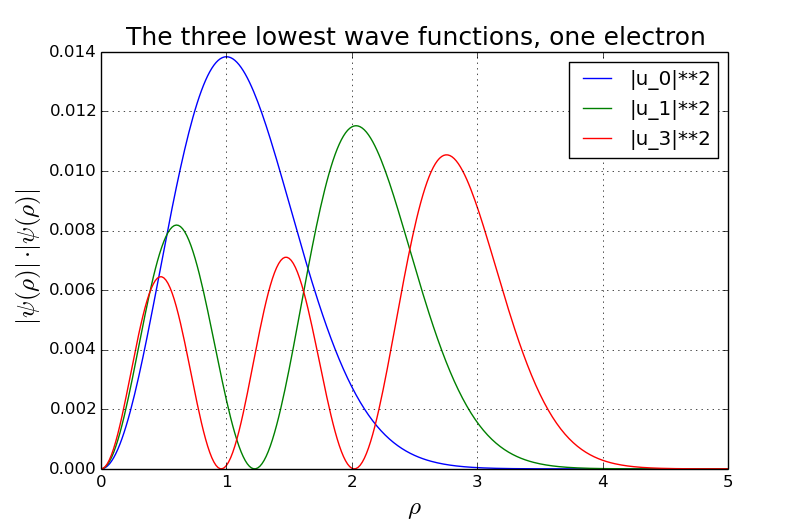
\includegraphics[scale=0.6]{wavefunc_one}\par
Figure 1: Plot of the wave functions of the three lowest states for the single electron system
\par
\vspace{5mm}

\subsubsection{Accuracy of the lowest eigenvalue vs N and $\rho_{max}$}\par
\vspace{3mm}
We experimented with how the precision of the lowest eigenvalue $\lambda_0$ changed with number of grid point used and the chosen value og $\rho_{max}$. The results are presented in Table 2.
\par
\vspace{3mm}


Table 2: Calculated value of the lowest eigenvalue $\lambda_0$, compared with number of grid points N and chosen value of $\rho_{max}$
\par
\vspace{2mm}

\begin{tabular}{|c|c|c|}\hline
     {\bf N, number of grid points} & {\bf Calculated value of $\lambda_0$ } & {\bf Value of $\rho_{max}$} \\ \hline
     5 & 9.82996 & 1\\
     100 & 10.1504 & 1\\
     350 & 10.1511 & 1\\ \hline
     5 & 2.68672 & 5\\
     100 & 2.99922 & 5\\
     350 & 2.99994 & 5\\ \hline
     5 &  4.49479 & 10\\
     100 & 2.99687  & 10\\
     350 & 2.99974 & 10 \\ \hline
  
\end{tabular}\par
\par
\vspace{3mm}

\subsubsection{Number of similarity transforms needed}
\par
\vspace{2mm}

We experimented with how the number of iterations needed to transform the matrix A into a diagonal matrix D changed with the number of grid points we used. The results are presented in Table 3.
\par
\vspace{3mm}


Table 3: Number of iterations needed to transform A into a diagonal matrix D, our tolerance is $\epsilon = 10^{-8}$
\par
\vspace{3mm}
\begin{tabular}{|c|c|c|}\hline
     {\bf N, number of grid points} & {\bf Number of iterations}\\ \hline
     5 & 14\\
     50 & 3862\\
     100 & 16182\\
     200 & 65920\\
     350 & 204523 \\ 
     400 & 268235\\\hline
\end{tabular}\par
  

\par
\vspace{5mm}

\subsection{Two electron system}
\par
\vspace{3mm}

\subsubsection{Plot of the wave functions}
\par
\vspace{3mm}

We plotted the wave functions of the three lowest states for the two-electron system, and varied the "frequency" of the potential. For $\omega = [0.01, 0.5, 1, 5]$, the resulting plots are shown in Figure 2-5. 
\par
\vspace{3mm}

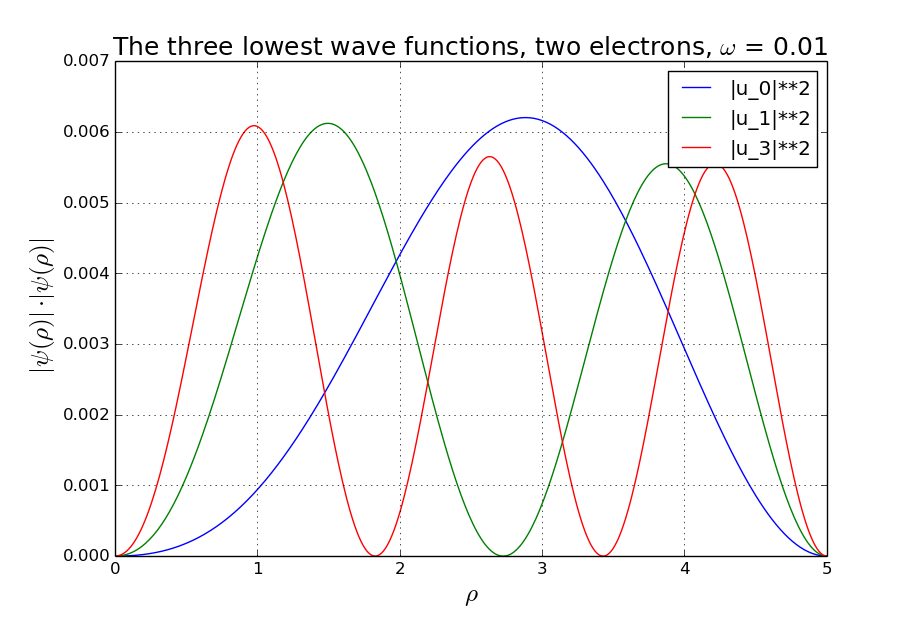
\includegraphics[scale=0.5]{wavefunc_two_omega=0_01}\par
\vspace{1mm}
Figure 2: Plot of the wave functions of the three lowest states for the two electron  system, with the "frequency" $\omega$ = 0.01
\par
\vspace{7mm}

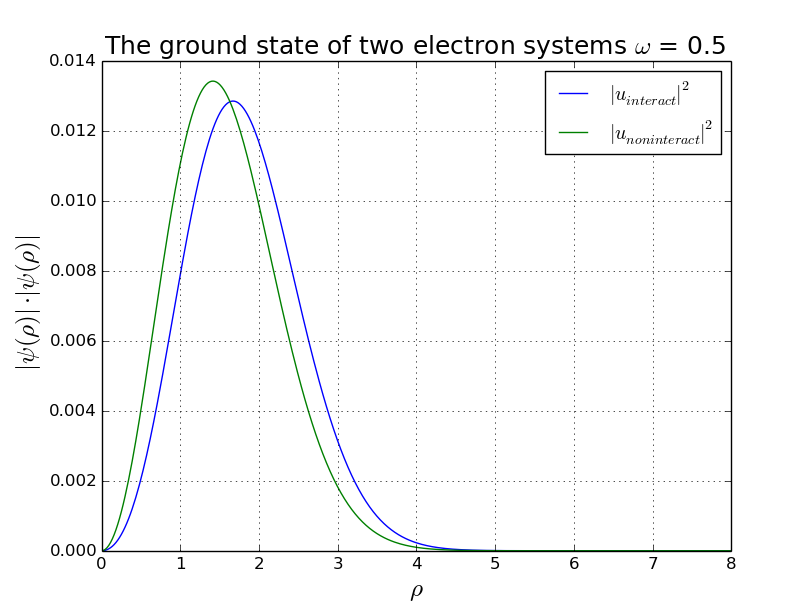
\includegraphics[scale=0.55]{wavefunc_two_omega=0_5}\par
\vspace{1mm}
Figure 3: Plot of the wave functions of the three lowest states for the two electron  system, with the "frequency" $\omega$ = 0.5
\par
\vspace{7mm}

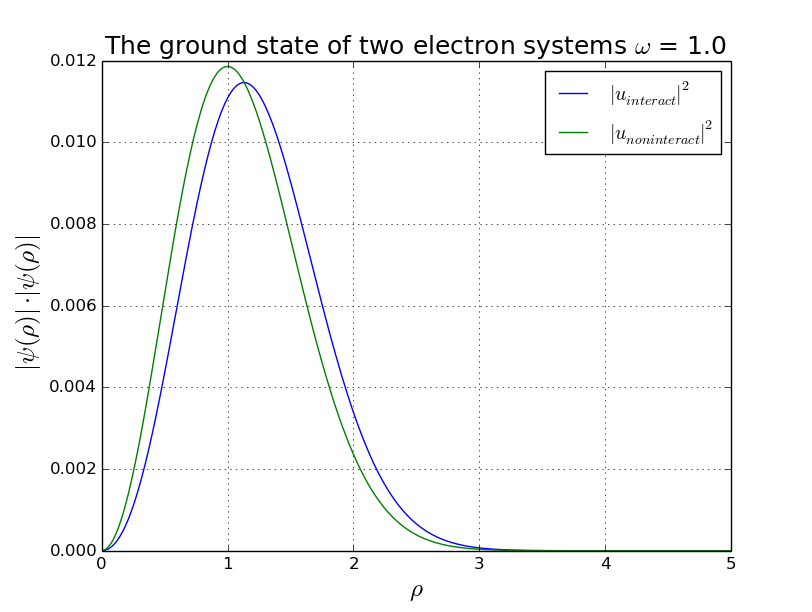
\includegraphics[scale=0.65]{wavefunc_two_omega=1}\par
\vspace{1mm}
Figure 4: Plot of the wave functions of the three lowest states for the two electron  system, with the "frequency" $\omega$ = 1
\par
\vspace{7mm}

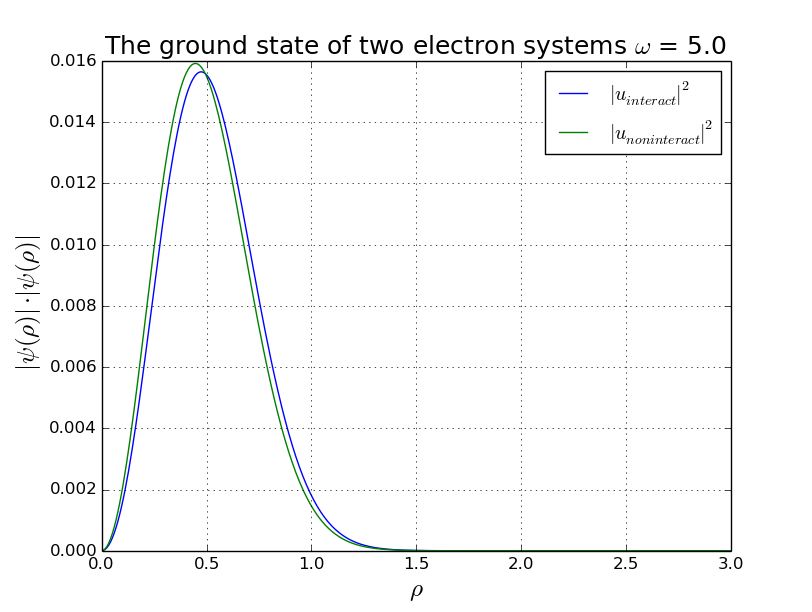
\includegraphics[scale=0.6]{wavefunc_two_omega=5}\par
\vspace{1mm}
Figure 5: Plot of the wave functions of the three lowest states for the two electron  system, with the "frequency" $\omega$ = 5
\par
\vspace{7mm}

\section{Discussion}


\section{Conclusion}
\section{References}
\begingroup
\renewcommand{\section}[2]{}
\begin{thebibliography}{}
\bibitem{MHJ15}
  Morten Hjorth-Jensen.
  Computational Physics, Lecture Notes Fall 2015.
  Department of Physics, University of Oslo.
  August 2015.

\end{thebibliography}
\endgroup
\section{Code attachment}
\end{document}
